\documentclass[sensors,article,submit,moreauthors,pdftex]{Definitions/mdpi}

\firstpage{1}
\makeatletter
\setcounter{page}{\@firstpage}
\makeatother
\pubvolume{xx}
\issuenum{1}
\articlenumber{5}
\pubyear{2026}
\copyrightyear{2026}
\history{Received: date; Accepted: date; Published: date}

\graphicspath{{figures/}}
\DeclareGraphicsExtensions{.pdf,.png,.eps}

\usepackage{amsmath}
\usepackage{booktabs}
\usepackage{subcaption}
\usepackage{multirow}
\usepackage{siunitx}

\Title{AERIS: Environment-Aware Hierarchical Routing for Reliable Wireless Sensor Networks under Realistic Channels}

\Author{Xiaobo Zhang $^{1}$, Kangrui Li $^{1,}$* and Junyi Lin $^{1}$}
\AuthorNames{Xiaobo Zhang, Kangrui Li and Junyi Lin}
\address{$^{1}$ \quad Faculty of Automation, Guangdong University of Technology, Guangzhou 510006, China}
\corres{Correspondence: 1403073295@mails.gdut.edu.cn}

\abstract{This study evaluates AERIS, a lightweight hierarchical routing protocol for wireless sensor networks under realistic channel conditions. The primary metric is \texttt{pdr\_expected} (base-station delivered packets divided by expected source packets). In publication-tier multi-environment experiments at 100 nodes (4 environments, 30 seeds each), AERIS achieves the highest packet delivery ratio among LEACH, PEGASIS, HEED, and TEEN in all evaluated environments. In scalability experiments (100--1000 nodes, 550 seeds each), AERIS ranks first in indoor\_factory, outdoor\_urban, and outdoor\_suburban, while PEGASIS remains higher in indoor\_office at all tested scales. Ablation results show environment-dependent module contribution: Gateway is significantly positive in three environments and near-neutral in indoor\_office; CAS does not show a consistent positive marginal effect. Hop-based latency analysis shows AERIS near two hops, whereas PEGASIS remains above 31 hops due to chain traversal. These results support a scoped conclusion: AERIS is suitable for reliability-oriented deployments across heterogeneous channels, but it is not a universal best protocol across all environments and scales.}

\keyword{wireless sensor networks; reliable routing; hierarchical protocol; packet delivery ratio; scalability; reproducible evaluation}

\begin{document}

\section{Introduction}
Wireless sensor network routing is classically optimized for energy reduction, but practical deployments also require stable delivery under heterogeneous channels. This creates a multi-objective tension among reliability, hop-based latency, and energy use. Existing protocols represent distinct operating points: LEACH emphasizes short paths to cluster heads, PEGASIS emphasizes chain-based energy efficiency, HEED emphasizes distributed head selection, and TEEN emphasizes event-triggered reporting.

AERIS is designed as a lightweight hierarchical protocol that prioritizes reliability under realistic channel variability. The design objective is not universal dominance, but robust performance across multiple channel environments while maintaining deployability on resource-constrained nodes.

\section{Related Work}
Classical WSN protocols (LEACH, PEGASIS, HEED, TEEN) provide foundational routing mechanisms but show different failure modes under harsh channels and larger scales. Chain-based aggregation can reduce per-hop transmission effort but increases end-to-end hop count. Cluster-based approaches can reduce hop count but may become sensitive to uplink quality and head placement.

Recent adaptive or learning-based methods improve specific settings but often require heavier runtime or training overhead. In this manuscript, the focus is a rule-based protocol with explicit reproducibility constraints and file-level provenance.

\section{System Model and Protocol}
\subsection{Metric Definition}
The primary metric is
\begin{equation}
\mathrm{PDR}_{\mathrm{expected}} = \frac{\mathrm{bs\_delivered}}{\mathrm{source\_packets\_expected}}.
\end{equation}
All publication conclusions in this draft are based on this metric.

\subsection{AERIS Architecture}
AERIS combines three components:
\begin{enumerate}
\item Context-Adaptive Switching (CAS) for mode control,
\item Skeleton backbone for hierarchical forwarding,
\item Gateway coordination for CH-to-BS reinforcement.
\end{enumerate}
Gateway candidate scoring follows a weighted rule
\begin{equation}
\mathrm{Score}_i = \alpha E_i + \beta C_i + \gamma L_i,
\end{equation}
where $E_i$ is residual energy, $C_i$ is centrality, and $L_i$ is link quality.

\section{Experimental Setup}
\subsection{Publication-Tier Settings}
\begin{itemize}
\item Simulator: Python implementation with logged provenance.
\item Channel environments: indoor\_office, indoor\_factory, outdoor\_urban, outdoor\_suburban.
\item Default node count: 100.
\item Seeds for multi-environment and ablation: 30 independent seeds.
\item Seeds for scalability: 550 independent seeds.
\item Baselines: LEACH, PEGASIS, HEED, TEEN.
\end{itemize}

\subsection{Evidence Files}
The analysis in this draft is grounded in:
\begin{itemize}
\item \texttt{results/mega\_experiments/env\_sensitivity\_20260207\_205317.json}
\item \texttt{results/mega\_experiments/ablation\_diag\_multi\_20260207\_205448.json}
\item \texttt{results/mega\_experiments/scalability\_4env\_550\_20260211\_103738\_descriptive.csv}
\item \texttt{results/mega\_experiments/scalability\_4env\_550\_20260211\_103738\_significance.csv}
\item \texttt{results/mega\_experiments/latency\_hop\_v3\_20260211\_stats.csv}
\item \texttt{results/mega\_experiments/latency\_hop\_v3\_20260211\_significance.csv}
\item \texttt{results/mega\_experiments/energy\_lifetime\_stats.csv}
\item \texttt{ns3\_validation/results/ns3\_multienv\_stats.csv}
\item \texttt{ns3\_validation/results/ns3\_multienv\_significance.csv}
\end{itemize}

\section{Results}
\subsection{Multi-Environment Comparison at 100 Nodes (n=30)}
\begin{table}[H]
\caption{PDR by environment at 100 nodes (mean +/- std).}
\label{tab:pdr100}
\centering
\begin{tabular}{lccccc}
\toprule
Environment & AERIS & LEACH & PEGASIS & HEED & TEEN \\
\midrule
indoor\_office   & 0.9739+/-0.0047 & 0.5543+/-0.0401 & 0.9078+/-0.0166 & 0.9371+/-0.0076 & 0.8222+/-0.0044 \\
indoor\_factory  & 0.6031+/-0.0258 & 0.1614+/-0.0209 & 0.1928+/-0.0255 & 0.2326+/-0.0263 & 0.3113+/-0.0245 \\
outdoor\_urban   & 0.3745+/-0.0354 & 0.0552+/-0.0127 & 0.0542+/-0.0117 & 0.0635+/-0.0121 & 0.1201+/-0.0183 \\
outdoor\_suburban& 0.7451+/-0.0193 & 0.2703+/-0.0272 & 0.3382+/-0.0329 & 0.4221+/-0.0313 & 0.4752+/-0.0236 \\
\bottomrule
\end{tabular}
\end{table}

At 100 nodes, AERIS ranks first in all four tested environments.

\begin{figure}[H]
\centering
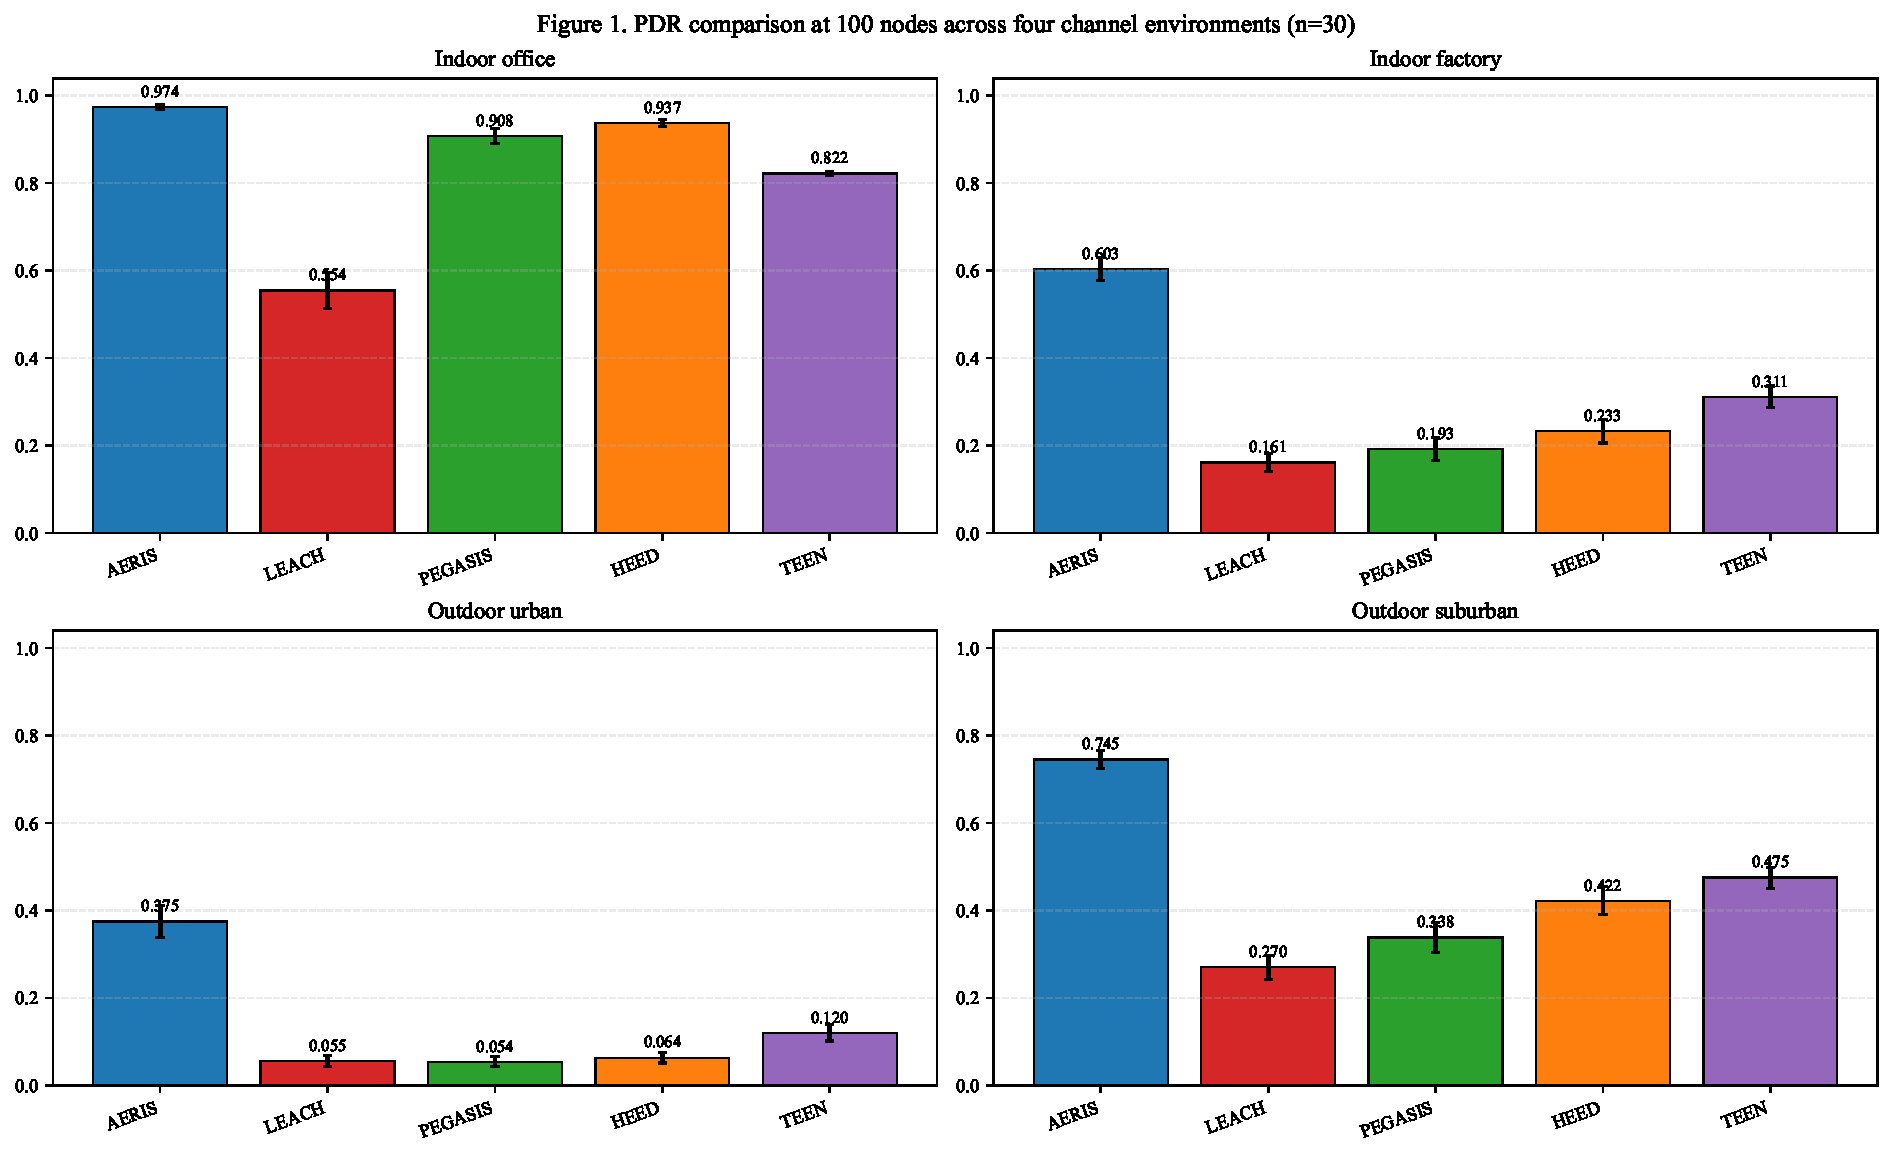
\includegraphics[width=0.95\textwidth]{fig1_env_pdr_panel_20260210_mdpi.pdf}
\caption{PDR comparison panel at 100 nodes (4 environments, n=30).}
\label{fig:env_panel}
\end{figure}

\subsection{Ablation: Environment-Dependent Effects (n=30)}
\begin{table}[H]
\caption{Full vs no\_gateway PDR (mean +/- std).}
\label{tab:ablation_gateway}
\centering
\begin{tabular}{lccc}
\toprule
Environment & Full & no\_gateway & Delta (no\_gateway - full) \\
\midrule
indoor\_office    & 0.9739+/-0.0047 & 0.9741+/-0.0036 & +0.0002 \\
indoor\_factory   & 0.6031+/-0.0258 & 0.5806+/-0.0215 & -0.0225 \\
outdoor\_urban    & 0.3745+/-0.0354 & 0.3534+/-0.0301 & -0.0212 \\
outdoor\_suburban & 0.7451+/-0.0193 & 0.7306+/-0.0264 & -0.0146 \\
\bottomrule
\end{tabular}
\end{table}

Gateway is positive in three environments and near-neutral in indoor\_office. CAS is not consistently positive across environments.

\begin{figure}[H]
\centering
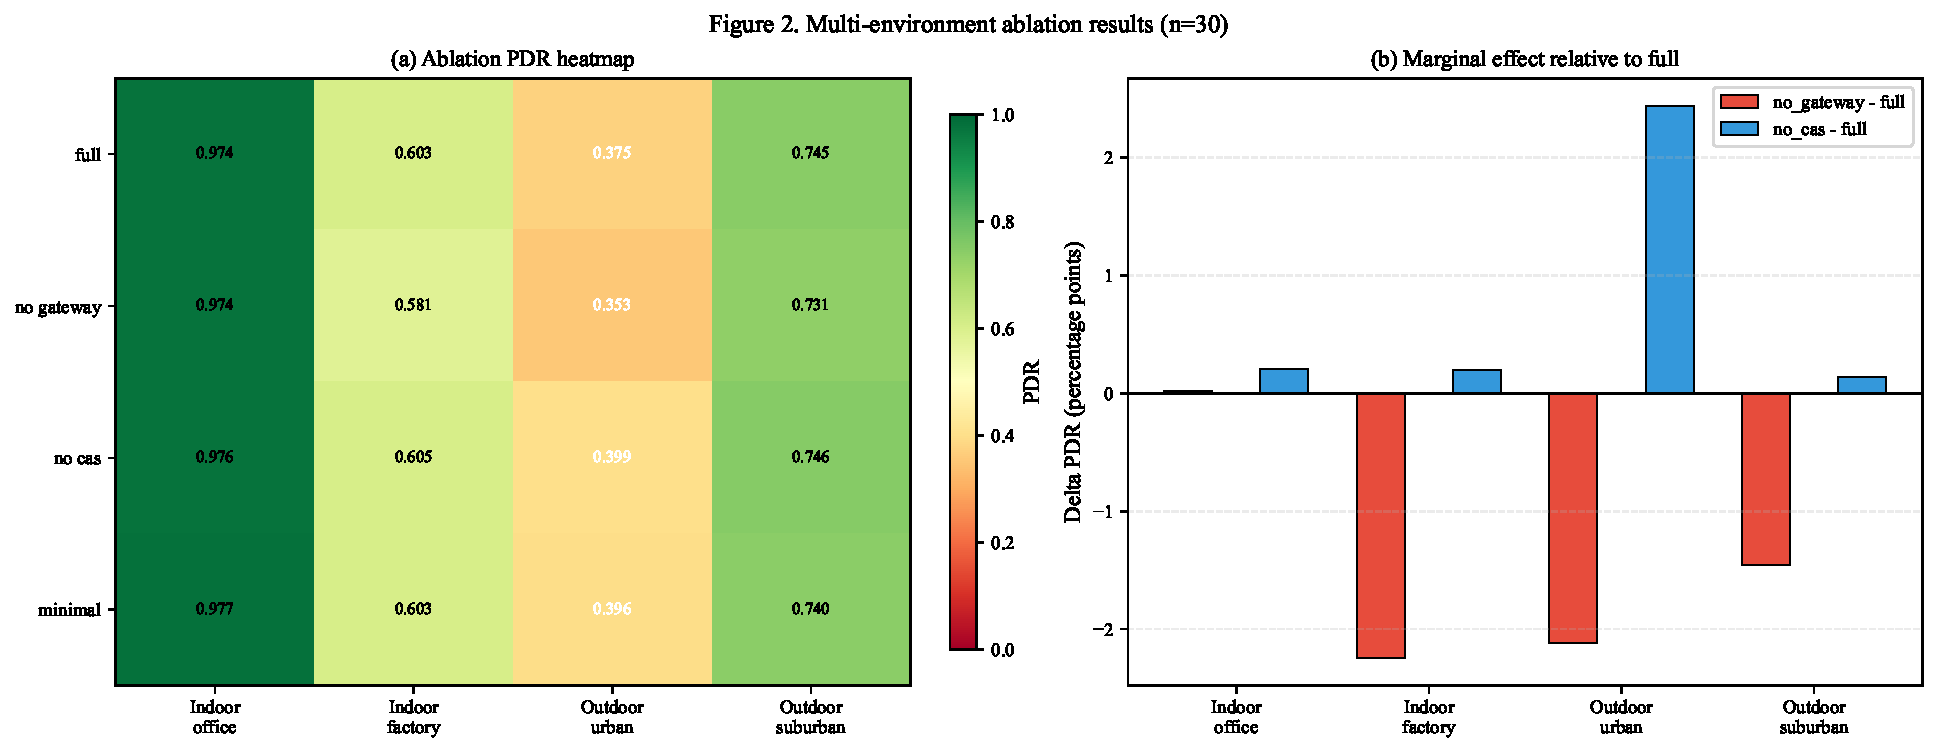
\includegraphics[width=0.95\textwidth]{fig2_ablation_panel_20260210_mdpi.pdf}
\caption{Ablation panel: heatmap and marginal effects (n=30).}
\label{fig:ablation_panel}
\end{figure}

\subsection{Scalability (100--1000 Nodes, n=550)}
\begin{table}[H]
\caption{PDR ranking at 1000 nodes.}
\label{tab:scale1000}
\centering
\begin{tabular}{lcccccc}
\toprule
Environment & AERIS & LEACH & PEGASIS & HEED & TEEN & AERIS rank \\
\midrule
indoor\_office    & 0.9899 & 0.9902 & 0.9992 & 0.9912 & 0.9922 & 5th \\
indoor\_factory   & 0.9900 & 0.4076 & 0.6102 & 0.3704 & 0.4926 & 1st \\
outdoor\_urban    & 0.9899 & 0.1566 & 0.2617 & 0.1291 & 0.1945 & 1st \\
outdoor\_suburban & 0.9900 & 0.5952 & 0.7871 & 0.5544 & 0.6893 & 1st \\
\bottomrule
\end{tabular}
\end{table}

AERIS is first in 3/4 environments across scales, while PEGASIS is higher in indoor\_office.

\begin{figure}[H]
\centering
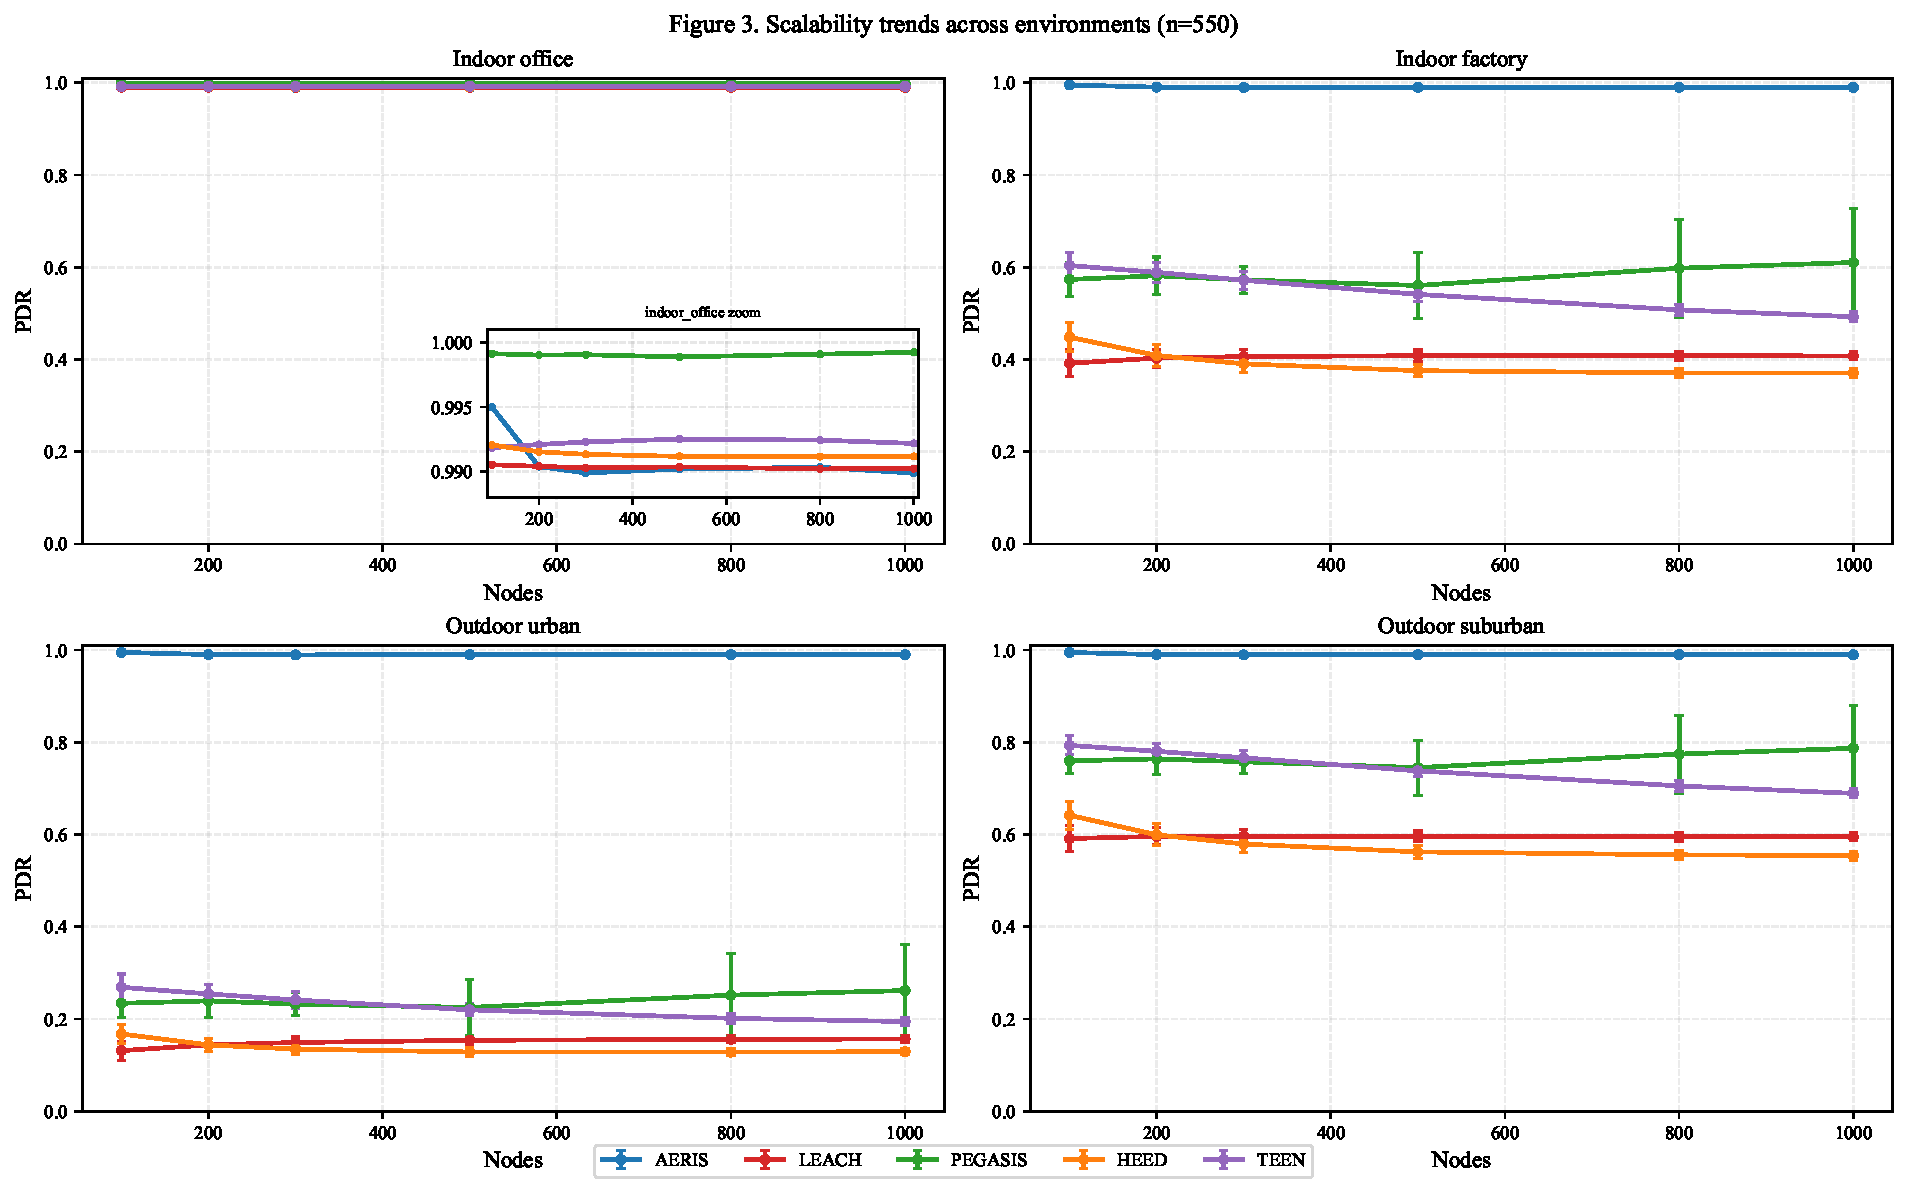
\includegraphics[width=0.95\textwidth]{fig3_scalability_panel_20260210_mdpi.pdf}
\caption{Scalability trends over node counts (n=550).}
\label{fig:scalability_panel}
\end{figure}

\subsection{Hop-Based Latency and Trade-offs}
At 100 nodes (n=30), AERIS stays near two hops (1.97--1.99), while PEGASIS remains above 31 hops due to chain traversal. LEACH and TEEN show lower average hops because of direct-to-BS transmissions in their protocol behavior.

\begin{figure}[H]
\centering
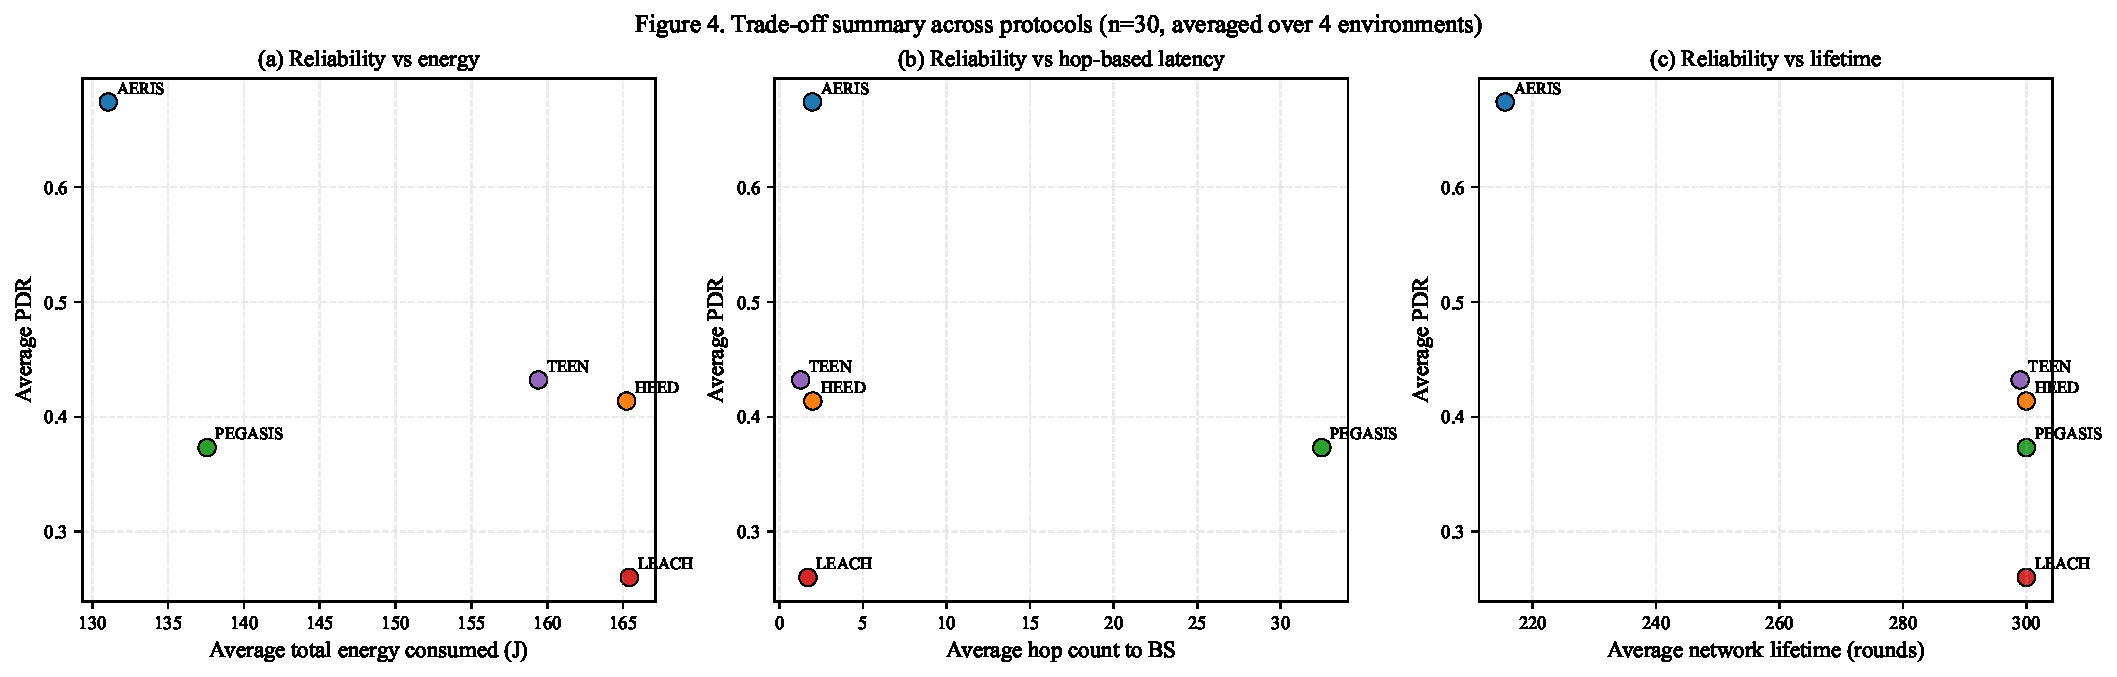
\includegraphics[width=0.95\textwidth]{fig4_tradeoff_panel_20260210_mdpi.pdf}
\caption{Trade-off panel from publication-tier data: reliability, energy, hop-based latency, and lifetime.}
\label{fig:tradeoff_panel}
\end{figure}

\subsection{NS-3 Trend Validation (AERIS vs LEACH, n=30)}
NS-3 validation is used as a cross-platform trend check rather than a numerical-equivalence proof. Under aligned multi-environment settings, AERIS is directionally not lower than LEACH in all tested environment-scale cells. At 100 nodes, significance is confirmed in 3/4 environments (indoor\_factory, outdoor\_urban, outdoor\_suburban), while indoor\_office remains non-significant. In the 300/500-node extension, all 8 environment-scale comparisons are significant after Holm correction.

\begin{table}[H]
\caption{NS-3 trend-level validation at 100 nodes (AERIS vs LEACH, n=30; metric=\texttt{pdr\_expected}).}
\label{tab:ns3_trend}
\centering
\begin{tabular}{lccccc}
\toprule
Environment & AERIS & LEACH & Delta & Holm-corrected $p$ & Significance \\
\midrule
indoor\_office    & 0.9202 & 0.9185 & +0.0017 & 1.00 & no \\
indoor\_factory   & 0.5996 & 0.5299 & +0.0698 & $<10^{-20}$ & yes \\
outdoor\_urban    & 0.2070 & 0.1891 & +0.0179 & $<10^{-4}$ & yes \\
outdoor\_suburban & 0.7769 & 0.6963 & +0.0806 & $<10^{-25}$ & yes \\
\bottomrule
\end{tabular}
\end{table}

Scope note: this NS-3 block supports trend consistency only. The manuscript does not claim cross-platform numerical equivalence. Across 5 node counts and 4 environments, 18/20 AERIS-vs-LEACH comparisons are significant.

\section{Discussion}
The results support a scoped positioning. AERIS is strong for reliability across heterogeneous channels but is not universally best in every environment-scale pair. The indoor\_office scalability result is a stable counterexample where PEGASIS is higher. This should remain explicit in manuscript claims.

Energy interpretation requires care: lower total energy can co-occur with shorter lifetime because some protocols stop earlier. Therefore, reliability-energy claims should be expressed as trade-offs under fixed evaluation conditions, not as universal dominance.

\section{Limitations and Future Work}
\begin{itemize}
\item Current evidence is simulator-based.
\item NS-3 trend-level publication gate is completed; numerical-equivalence gate is intentionally not claimed due platform-depth differences.
\item Additional topology families (corridor, hotspot) and hardware-in-the-loop validation remain pending.
\end{itemize}

\section{Conclusion}
AERIS provides a reliability-oriented routing option for heterogeneous WSN channels. Under publication-tier Python evaluation, it achieves the highest PDR in all four environments at 100 nodes and maintains first rank in three of four environments at larger scales. NS-3 validation confirms trend consistency for AERIS versus LEACH across four environments but is used as trend-level evidence only. Gateway effects are environment-dependent, and CAS effects are mixed. The manuscript should therefore retain strict scope language and avoid universal claims.

\authorcontributions{Conceptualization, X.Z. and K.L.; methodology, K.L. and J.L.; software, K.L.; validation, X.Z. and J.L.; writing---original draft preparation, K.L.; writing---review and editing, X.Z.; supervision, X.Z.}
\funding{This research received no external funding.}
\institutionalreview{Not applicable.}
\informedconsent{Not applicable.}
\dataavailability{Data and scripts are available in the project repository under results/mega\_experiments and scripts/.}
\conflictsofinterest{The authors declare no conflict of interest.}

\end{document}

